% Question  ##################################################################################################################
\section{Question 2}\label{ssec:pt1q2}
\textbf{Modern or mean-variance portfolio theory (MPT) is a major cornerstone of financial theory. Based
on this theoretical breakthrough the Nobel Prize in Economics was awarded to its inventor, Harry
Markowitz, in 1990. Using the data from Question 1, we need to investigate the right allocation
across a portfolio made up of 3 investments, S\&P500, FTSE 100 and Gold (SPDR). }

% END Question  ##############################################################################################################

% Question (i) ###############################################################################################################

\subsection{Q2 (i)}\label{sssec:pt1q2i}
\textbf{In question 1, you identified the individual expected return and volatility of the 3 investments
separately. Calculate the expected return and volatility of the portfolio, considering equal weight for the 3 investments. }

\noindent
Code for this question can be found in the notebook in section 'Question 2 (i)'. Before calculating both measurements for the portfolio, it was noted that there is some discrepancy between the dates of the assets. The dates of S\&P500 and Gold were not matching with the dates for the FTSE100 index. To solve this dates were aligned to capture more accurate measurements. 

\noindent
To calculate the annualized return and volatility for the portfolio a new function called ‘ann\_ret\_vol’ was created in the ‘fintech’ library as shown in Fig.~\ref{fig:annretport}. This was later called from the notebook cell. As shown, this function takes three parameters. For first parameter a new pandas dataframe with the log returns for each asset was created (each column has the log returns for each asset). After doing so an equal weight was set as a numpy array and passed as a parameter. In this task it was assumed that a year has 250 days. 

\begin{figure}[H]
\centering
  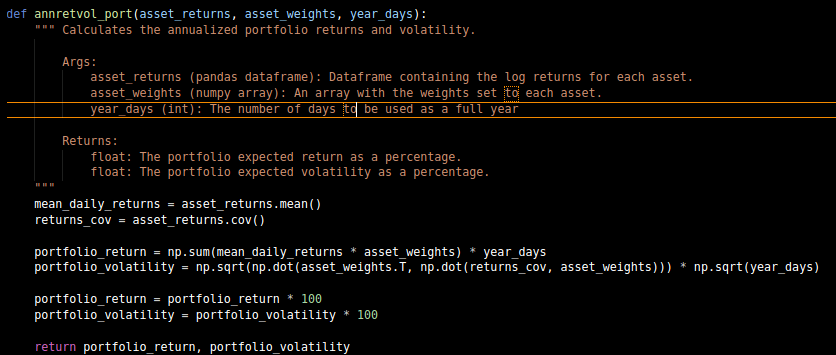
\includegraphics[scale = .55]{imgs/annvolret.png}
  \caption{Function to measure expected returns and volatility for portfolio.}
  \label{fig:annretport}
\end{figure}

\noindent
To calculate the expected return for the portfolio the weighted sum of the mean return for each asset was taken and multiplied by the number of days (to annualize) as shown in Eq.~\ref{eq:portret}.  

\begin{equation} \label{eq:portret}
   E(r) = \Sigma w_i k_i
\end{equation}

\noindent
On the other hand, calculating portfolio risk is a bit more complicated than taking the sum of the weighted volatility of each asset. To calculate the volatility of the portfolio, first we need to find the covariance between the asset's returns, since the risk of an asset may be correlated with another asset. Eq.~\ref{eq:portvol} shows how to calculate volatility for a portfolio with two assets but this can be easily extended to three assets when writing it in code as shown in Fig.~\ref{fig:annretport}. The final measurements for the portfolio are shown in Fig.~\ref{fig:portretvolresults}. 

\begin{equation} \label{eq:portvol}
   \sigma = \sqrt{(w_1^2 \sigma_1^2) + (w_2^2 \sigma_2^2) + 2 (w_1) (w_2) (Corr(R_1, R_2) \sigma_1 \sigma_2)}     
\end{equation}

\begin{figure}[H]
\centering
  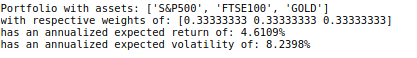
\includegraphics[scale = .75]{imgs/portretvolresults.png}
  \caption{Results for portfolio volatility and returns.}
  \label{fig:portretvolresults}
\end{figure}

% END Question (i) ###########################################################################################################

% Question (ii) ##############################################################################################################

\subsection{Q2 (ii)}\label{sssec:pt1q2ii}

\textbf{Investigate different portfolio expected return and volatility by simulating different random
weights of your investments (2000 simulations). Assume that all weights have to be $>0$ and that the
sum of all weights should be equal to 1. Create a plot showing the expected return (y-axis) and volatility (x-axis) for different/random portfolio weights.}

\noindent
The code for this simulation can be found in 'Question 2 (ii)' in the notebook and a function called 'annretvol\_port\_rand' was created in the 'fintech' library to simulate different weights for a portfolio as shown in Fig.~\ref{fig:portsimulationcode}. The plot shown in Fig.~\ref{fig:portsimulation} shows the expected return (y-axis) and the volatility (x-axis) for these simulations. 

\begin{figure}[H]
\centering
  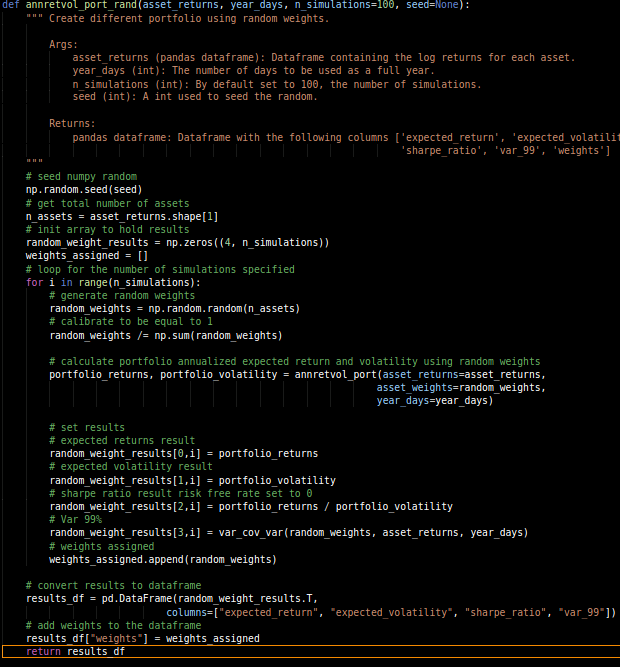
\includegraphics[scale = .65]{imgs/port_sim_code.png}
  \caption{Function to generate portfolio returns and volatility using random weights.}
  \label{fig:portsimulationcode}
\end{figure}

\begin{figure}[H]
\centering
  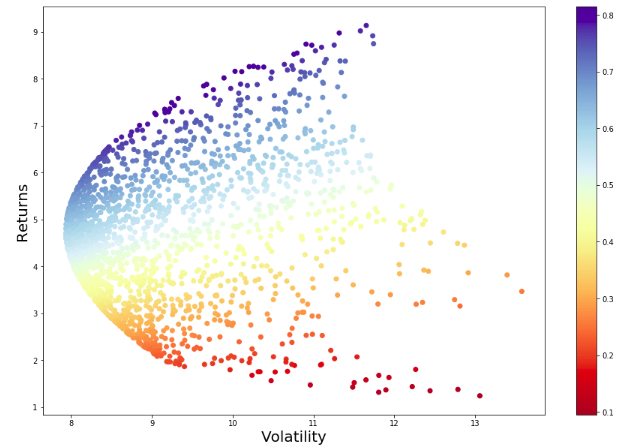
\includegraphics[scale = .65]{imgs/port_simulation.png}
  \caption{Portfolio returns and volatility using random weights (2000 Simulations).}
  \label{fig:portsimulation}
\end{figure}

% END Question (ii) ##########################################################################################################

% Question (iii) #############################################################################################################

\subsection{Q2 (iii)}\label{sssec:pt1q2iii}
\textbf{Using an optimisation library (e.g. using solver in excel or an optimisation library in python),
identify the two portfolios that will return (a) the highest Sharpe ratio and (b) the lowest Value at 
Risk. For the Sharpe ratio, assume that the risk free rate is zero. Using the plot in question (ii), indicate the position of these two portfolios.}

\noindent
\textbf{In your answers explain the method/steps used.}

\noindent
The code for this question is shown in 'Question 2 (iii)' and as an optimization library a third party library called 'scipy.optimize' \cite{python:scipy} was utilised for this process. For the highest Sharpe ratio a function called 'max\_sharperatio\_port' was created in the 'fintech' library as shown in Fig.~\ref{fig:maxsharperatio}. 

\noindent
In this function the third party library described, is used to minimize the negative Sharpe ratio which gives us the portfolio with the highest Sharpe ratio. The function which is being minimized is shown in Fig.~\ref{fig:negsharperatio}. After the function finds the minimum, the values described in the code comments in Fig.~\ref{fig:maxsharperatio} are returned. The final output for the highest Sharpe Ratio is shown in Fig.~\ref{fig:maxsharperatioresults}. 

\begin{figure}[H]
\centering
  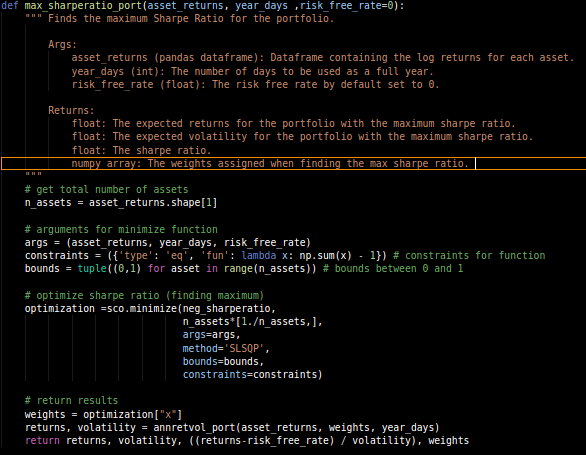
\includegraphics[scale = .65]{imgs/maxsharpefunc.png}
  \caption{Function used to find the maximum Sharpe Ratio for a portfolio.}
  \label{fig:maxsharperatio}
\end{figure}

\begin{figure}[H]
\centering
  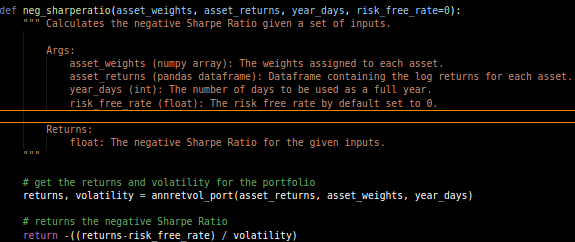
\includegraphics[scale = .65]{imgs/negsharperatio.png}
  \caption{The function being minimized to find the maximum Sharpe Ratio.}
  \label{fig:negsharperatio}
\end{figure}

\begin{figure}[H]
\centering
  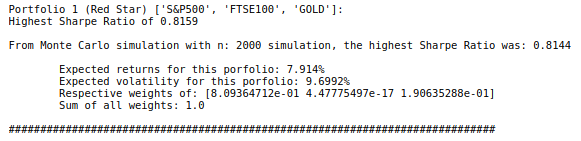
\includegraphics[scale = .75]{imgs/maxsharperatioresults.png}
  \caption{The results for the portfolio with the max Sharpe Ratio.}
  \label{fig:maxsharperatioresults}
\end{figure}

\noindent
For the other measurement, which is the lowest VaR(99\%) for the portfolio, another function was created called ‘min\_var\_port’ in the ‘fintech’ library as shown in Fig.~\ref{fig:minvarport}. The same optimization library used to get the previous measurement was utilised.   

\begin{figure}[H]
\centering
  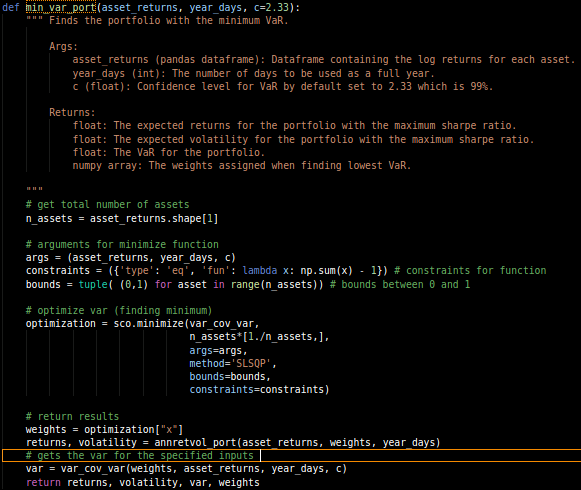
\includegraphics[scale = .75]{imgs/minvarport.png}
  \caption{Function used to get the minimum VaR for a portfolio.}
  \label{fig:minvarport}
\end{figure}

\noindent
Similarly, to the previous function a value/function is being minimized to get the desired output. The function being minimized is the computed VaR using the covariance variance approach. This function is shown in Fig.~\ref{fig:minimizeminvarport}. After the function finds the minimum, the values described in the code comments in Fig.~\ref{fig:minvarport} are returned. The final output for the lowest VaR(99\%) is shown in Fig.~\ref{fig:minvarresults}.

\noindent 
Finally these measurements were plotted on the same plot used in (ii) where the red star indicates the portfolio with the maximum Sharpe Ratio and the green star indicates the portfolio with the lowest VaR(99\%). This plot is shown in Fig.~\ref{fig:portsimbest}.

\begin{figure}[H]
\centering
  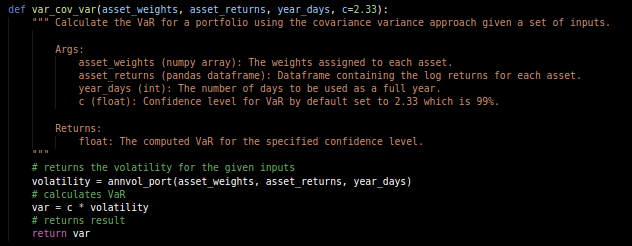
\includegraphics[scale = .75]{imgs/varminimize.png}
  \caption{The function being minimized to find the lowest VaR.}
  \label{fig:minimizeminvarport}
\end{figure}

\begin{figure}[H]
\centering
  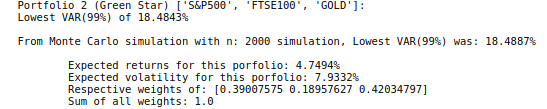
\includegraphics[scale = .75]{imgs/minvarresults.png}
  \caption{The results for the portfolio with the lowest VaR.}
  \label{fig:minvarresults}
\end{figure}

\begin{figure}[H]
\centering
  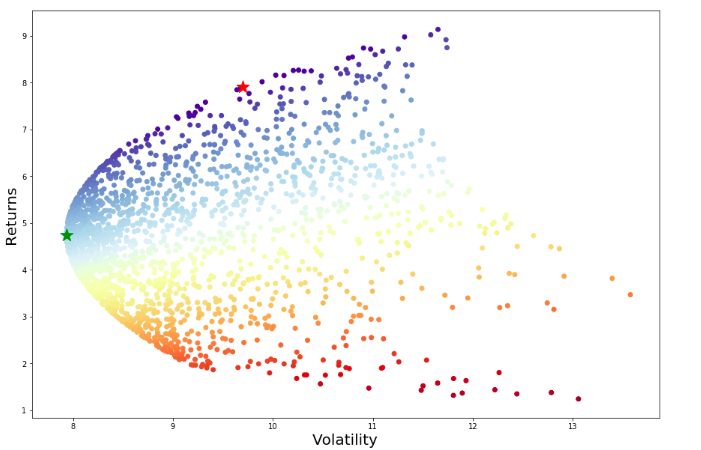
\includegraphics[scale = .65]{imgs/port_simulation_best.png}
  \caption{The portfolio with the Highest Sharpe Ratio (Red Star) and with the lowest VaR(99\%) (Green Start) on the plot used in (ii).}
  \label{fig:portsimbest}
\end{figure}

% END Question (iii) #########################################################################################################